\documentclass[UTF8]{article}
\usepackage{ctex}
\usepackage{graphicx}
\usepackage{amssymb}

\title{无类型的$\lambda$-演算\\[2ex]\begin{large}读书笔记\end{large}}
\author{许博}
\date{}

\begin{document}
\maketitle
	
\section{疑惑}
	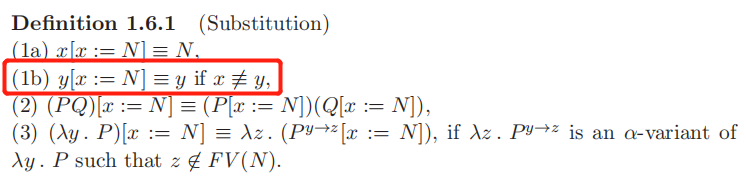
\includegraphics[width=0.93\linewidth]{"../imgs/1-1.png"}
	
	x 和 y 什么时候句法等同$\equiv$?
	
\section{函数的本质(essence)}

	在 $\lambda$-calculus 中,函数被表示为如 $\lambda x. x^2 + 1$ 的形式,. 的右边是表达式,$\lambda$x 表示在表达式中 x 是一个变量,同时 x 是该函数的形参。在函数调用时,传入的值跟随在函数之后以括号包裹,如 $(\lambda x. x^2 + 1)(3)$。
	
	总结出两个构造原则(construction principles)和一个求值规则(evaluation rule)。
	
\subsection{构造原则}

	\begin{enumerate}
		\item 抽象(Abstraction):由表达式 M 和变量 x 可以构造得到一个新的表达式:$\lambda x. M$,称之为 M 上 x 的抽象。
		\item 应用(Application):由表达式 M 和 N 可以构造表达式 $M N$,称之为 M 应用于 N。
	\end{enumerate}

	函数 $\lambda x. x^2$ 中,表达式 $x^2$ 不是一个函数,而是一个抽象的输出值,表示 x 的平方。与函数的区别在于,假设 x 是一个自然数,函数 $\lambda x. x^2$ 接收自然数返回自然数,而 $x^2$ 表示一个自然数。
	
\subsection{求值规则}
	
	函数求值的过程的形式化称为 $\beta$-规约($\beta$-reduction),使用替换(substitution)来进行计算,由中括号进行表示,如表达式 $M\left[x := N\right]$ 表示 M 中的 x 被替换成 N。
	
	$\beta$-规约:形如 $(\lambda x. M)N$ 的表达式可以被重写为表达式 $M\left[x := N\right]$,表达式 M 中的每一个 x 都会被替换成 N,从 $(\lambda x. M)N$ 到 $M\left[x := N\right]$ 的过程记为 $\beta$-规约。
	
\subsection{多参数}

	本书中,只考虑单参数的函数,在函数需要多个参数时,可以通过柯里化,使用单参数函数的复合来模拟多参数函数,如函数 $\lambda (x, y). (x^2 + y)$ 可以柯里化为函数 $\lambda x. (\lambda y. (x^2 + y))$,即为函数 g,在求值时,可以通过形如 $g(3)(5)$ 的方式来进行应用。

\section{$\lambda$-项(terms)}

	$\lambda$-演算中主要关心的部分是以最简单,最抽象的视角描述函数的行为,可以不考虑数,以及和数有关的操作,如加法等,剩下的部分为:
	
	\begin{enumerate}
		\item 变量(x, y, ...)
		\item 构造原则,抽象和应用
		\item 求值规则,$\beta$-规约
	\end{enumerate}
	
\subsection{$\Lambda$}

	$\lambda$-演算中的表达式被称为 $\lambda$-项,所有 $\lambda$-项的集合 $\Lambda$ 可以通过归纳的定义来构造,首先假设存在一个无限的变量集合 V,$V = \{x,y,z,...\}$。
	
	$\Lambda$ 的定义:
	\begin{enumerate}
		\item (变量)如果 $u \in V$,那么 $u \in \Lambda$
		\item (应用)如果 M 和 N $\in \Lambda$,那么 $(M N) \in \Lambda$
		\item (抽象)如果 $u \in V$ 以及 $M \in \Lambda$,那么 $(\lambda u. M) \in \Lambda$
	\end{enumerate}
	
	$\Lambda$ 以抽象语法的定义为:$\Lambda = V|(\Lambda\Lambda)|(\lambda V.\Lambda)$。
	
\subsection{$\lambda$-项的表示}

	\begin{enumerate}
		\item 使用字母 x, y, z 以及它们使用下标(subscript)和上标符(prime,$\prime$)的变体来表示 V 中的变量
		\item 使用 L, M, N, P, Q, R 以及它们的变体来表示 $\Lambda$ 中的元素
		\item 使用符号 $\equiv$ 表示两个 $\lambda$-项句法等同
	\end{enumerate}

	所以 $(x\ z) \equiv (x\ z)$,但是 $(x\ z) \not \equiv (x y)$,需要注意的是,$M \equiv N$ 表示 M 和 N 代表的实际的 $\lambda$-项句法等同。
	
\subsection{子项}

	记 $Sub(M)$ 为 M 中的子项的多重集(multiset),即相同的子项可以出现多次。Sub 的定义为:
	
	\begin{enumerate}
		\item (基础)$\forall x \in V. Sub(x) = \{x\}$
		\item (应用)$Sub((M N)) = Sub(M) \cup Sub(N) \cup \{(MN)\}$
		\item (抽象)$Sub((\lambda x.M)) = Sub(M) \cup {(\lambda x.M)}$
	\end{enumerate}
	
	如果 $L \in Sub(M)$,记 L 为 M 的一个子项。如 $Sub((\lambda x. (xx))) = \{((\lambda x. (xx)), xx, x, x\}$,其中 x 出现了两次,一次是 xx 中的第一个 x,一次是 xx 中的第二个 x。

\subsubsection{引理(lemma)}

	\begin{enumerate}
		\item (自反性,reflexivity)$\forall M \in \Lambda. M \in Sub(M)$
		\item (传递性,transitivity)由 ${L \in Sub(M)} \land {M \in Sub(N)}$ 可以得到 $L \in Sub(N)$
	\end{enumerate}

\subsubsection{真子项}

	如果 $\{L \in Sub(M)\} \land \{L \not \equiv\{M\}\}$,那么 L 是 M 的真子项。
	
\subsection{省略括号}

	\begin{enumerate}
		\item 最外层的括号可以省略:$MN \equiv (MN)$
		\item 应用是左结合的:$MNL \equiv ((MN)L)$
		\item 应用的优先级高于抽象:$\lambda x.MN \equiv \lambda x.(MN)$
		\item 同一 $\lambda$ 后出现的抽象是右结合的:$\lambda xy.M \equiv \lambda x. (\lambda y. M)$
	\end{enumerate}

\section{自由和约束(bound)变量}

	出现在 $\lambda$-项中的变量可以被分成三种:自由(free),约束(bound)和绑定(binding)。
	
	\begin{enumerate}
		\item 绑定变量,指直接出现在 $\lambda$ 之后的变量
		\item 约束变量,指出现在表达式中的绑定变量,如 $\lambda x. xy$ 中的第二个 x
		\item 自由变量,指出现在表达式中的非绑定变量,如 $\lambda x. xy$ 中的 y
	\end{enumerate}
	
\subsection{FV(L)}

	FV(L) 表示 $\lambda$-项 L 中的自由变量的集合,其定义为:
	\begin{enumerate}
		\item (变量)$FV(x) = \{x\}$
		\item (应用)$FV(MN) = FV(M) \cup FV(N)$
		\item (抽象)$FV(\lambda x. M) = FV(M) \ \{x\}$
	\end{enumerate}

	需要注意,$FV(x(\lambda x.xy)) = \{x, y\}$,尽管其中 x, y 都是自由变量,但是自由变量的 x 是 $x(\lambda x.xy)$ 中的第一个 x,而 y 之前的 x 依然是约束变量。

\subsection{组合子(combinator)}

	如果一个 $\lambda$-项 M 满足 $FV(M) = \emptyset$,称 M 是闭合的(closed),也可以将其称为是一个组合子。所有组合子的集合用 $\Lambda^0$ 表示。

\section{$\alpha$-变换(conversion)}

	$\lambda$-项中的绑定变量并不是必须的,如平方函数可以写作 $\lambda x. x^2$,也可以写作 $\lambda u. u^2$,都表示函数计算传入值的平方之后将得到的值作为输出值。变量名只是为了给传入的值提供一个临时的名字。因此在 $\lambda$-演算中,只有绑定变量(以及对应的约束变量)不同的 $\lambda$-项是相同的。

	定义关系 $\alpha$-变换或 $\alpha$-等价(equivalence)来形式化地描述这个过程:

	令 $M^{x\rightarrow y}$ 表示将 M 中所有的自由变量 x 替换为 y,重命名的关系使用符号 $=_{\alpha}$ 表示,则当 $y \notin FV(M)$ 以及 y 不是 M 中的绑定变量时,$\lambda x. M =_{\alpha} \lambda y. M^{x\rightarrow y}$。

	也即 $\lambda x. M$ 被重命名为 $\lambda y. M^{x\rightarrow y}$。

	$\alpha$-变换具有如下性质:
	\begin{enumerate} 
		\item (相容性,compatibility)如果 $M =_{\alpha} N$,那么 $ML =_\alpha NL, LM =_\alpha LN$,并且对于任意的 z,$\lambda z. M =_\alpha \lambda z. N$
		\item (自反性,reflexivity)$M =_\alpha M$
		\item (对称性,symmetry)如果 $M =_\alpha N$,那么 $N =_\alpha M$
		\item (传递性,transitivity)如果 $L =_\alpha M \land M =_\alpha N$,那么 $L =_\alpha N$
	\end{enumerate}

	如果 $M =_\alpha N$,则 M 和 N 称为 $\alpha$-可变换($\alpha$-convertible)或 $\alpha$-等价($\alpha$-equivalent)。M 被记为是 N 的一个 $\alpha$-变体($\alpha$-variant)。

\section{替换}

	替换 $\lambda$-项中的自由变量,它的定义如下:
	\begin{enumerate}
		\item $x[x:=N]\equiv N$
		\item 如果 $x \not \equiv{y}$,那么 $y[x:=N]\equiv y$
		\item $(PQ)[x:=N]\equiv (P[x:=N])(Q[x:=N])$
		\item 如果 $\lambda z. P^{y\rightarrow z}$ 是 $\lambda y.P$ 的一个 $\alpha$-变体,且 $z \notin FV(N)$,则 $(\lambda y. P)[x:=N]\equiv \lambda z.(P^{y\rightarrow z}[x:=N])$
	\end{enumerate}

	重命名可被看作是一种特殊的替换,如 $M^{x\rightarrow u} =_\alpha M[x:=u]$,如果重命名的条件满足的话。

	替换的顺序会影响 $\lambda$-项,如 $x[x:=y][y:=x]\equiv x$,但是 $x[y:=x][x:=y]\equiv y$。

	$M[x:=L]$ 不是一个合法的 $\lambda$-项,当替换执行完之后,所有的 $[x:=L]$ 都消失了以后所得到的才是 $\lambda$-项。

\subsection{引理}

	令 $x \not \equiv{y} \land x \notin FV(L)$:

	$M[x:=N][y:=L]\equiv M[y:=L][x:=N[y:=L]]$

\section{$\lambda$-项模 $\alpha$ 等价(module $\alpha$-equivalence)}

	$\alpha$-等价在项构造时会被保留,引理:

	令 $M_1 =_\alpha N_1 \land M_2 =_\alpha N_2$,则:
	\begin{enumerate}
		\item $M_1 N_1 =_\alpha M_2 N_2$
		\item $\lambda x. M_1 =_\alpha \lambda x. M_2$
		\item $M_1[x:=N_1]=_\alpha M_2[x:=N_2]$
	\end{enumerate}

	句法等同 $\equiv$ 现在包括 $\alpha$-等价 $=_\alpha$。

\subsection{Barendregt 约定}

	约定 $\lambda$-项中的绑定变量的名字都不相同,并且与其中出现的所有自由变量也不相同。

	如使用 $(\lambda xy.xz)(\lambda uv.v)$,而非 $(\lambda xy.xz)(\lambda xz.z)$。

\section{$\beta$-规约}

\subsection{单步 $\beta$-规约(one-step $\beta$-reduction,$\rightarrow_\beta$)}

	\begin{enumerate}
		\item (基础,Basis)$(\lambda x.M)N \rightarrow_\beta M[x:=N]$
		\item (相容性,compatibility)如果 $M \rightarrow_\beta N$,那么 $ML \rightarrow_\beta NL$,$LM \rightarrow_\beta LN$ 以及 $\lambda x.M\rightarrow_\beta \lambda x.N$
	\end{enumerate}

	形如 $(\lambda x.M)N$ 的 $\lambda$-项记为 redex(可规约的表达式,reducible expression),而规约后的 $M[x:=N]$ 记为 contractum。

\subsection{$\beta$-规约(零步或多步,$\twoheadrightarrow_\beta$)}

	如果存在 $n\ge 0$,有若干项 $M_0, ..., M_n$,且 $M_0 \equiv M, M_n \equiv N$,以及对于 $0 \le i < n$,有 $M_i \rightarrow_\beta M_{i+1}$,则有 $M \twoheadrightarrow_\beta N$。

	$\twoheadrightarrow_\beta$ 具有自反性以及传递性。

\subsection{$\beta$-变换($\beta$-conversion,$\beta$-equality,$=_\beta$)}

	如果存在 $n\ge 0$,有若干项 $M_0, ..., M_n$,且 $M_0 \equiv M, M_n \equiv N$,以及对于 $0 \le i < n$,有 $M_i \rightarrow_\beta M_{i+1}$ 或 $M_{i+1} \rightarrow_\beta M_i$,则有 $M =_\beta N$。

	对于 $(\lambda y.yv)z \rightarrow_\beta zv \leftarrow_\beta (\lambda x.zv)v$ 而言,也有 $(\lambda y.yv)z =_\beta (\lambda x.zv)v$。

	$=_\beta$ 具有自反性,对称性以及传递性。

\section{范式(normal forms)}

	定义:
	\begin{enumerate}
		\item 如果 M 不能进行 $\beta$-规约,则 M 是满足 $\beta$-范式($\beta$-nf)的
		\item 如果存在 N 使得 $M =_\beta N$,则称 M 具有 $\beta$-范式 N,或称 M 是可 $\beta$-常化($\beta$-normalising)的。
	\end{enumerate}

	记 M 的 $\beta$-范式为 M 的输出。

\subsection{引理}

	当 M 满足 $\beta$-范式,那么 $M \twoheadrightarrow_\beta N$ 隐含 $M \equiv N$。

\subsection{规约路径(reduction path)}

	\begin{enumerate}
		\item (M 的有限规约路径)一个有限 $\lambda$-项序列 $N_0, N_1, N_2, ..., N_n$,且 $N_0 \equiv M$ 以及对于 $0 \le i < n$ 有 $N_i \rightarrow_\beta N_{i+1}$
		\item (M 的无限规约路径)一个无限 $\lambda$-项序列 $N_0, N_1, N_2, ...$,且 $N_0 \equiv M$ 以及对于自然数 i 有 $N_i \rightarrow_\beta N_{i+1}$
	\end{enumerate}

\subsection{Weak/strong normalisation}

	\begin{enumerate}
		\item 如果存在 $\beta$-范式 N,使得 $M \twoheadrightarrow_\beta N$,称 M 为 weakly normalising
		\item 如果不存在以 M 出发的无限规约路径,则称 M 为 strongly normalising
	\end{enumerate}

	所有的 strongly normalising 的项都是 weakly normalising 的。

\subsection{Church-Rosser 定理}

	缩写为 CR,或称汇流(Confluence)定理

	假设对于给定的 $\lambda$-项 M,有 $M \twoheadrightarrow_\beta N_1$ 以及 $M \twoheadrightarrow_\beta N_2$,则存在一个 $\lambda$-项 $N_3$ 使得 $N_1 \twoheadrightarrow_\beta N_3$ 以及 $N_2 \twoheadrightarrow_\beta N_3$。

	通过 CR 定理可以得到一个结论,假设 $M =_\beta N$,则存在 L 使得 $M \twoheadrightarrow_\beta L$ 以及 $N \twoheadrightarrow_\beta L$。

\subsection{引理}

	\begin{enumerate}
		\item 如果 N 是 M 的 $\beta$-范式,那么 $M \twoheadrightarrow_\beta N$
		\item 一个 $\lambda$-项至多有一个 $\beta$-范式
	\end{enumerate}

	非正式表述如下:
	\begin{enumerate}
		\item 如果一个 $\lambda$-项有一个输出,则这个输出可以向前(forward)计算到达
		\item 一个计算的输出若存在则唯一
	\end{enumerate}

\section{不动点(fixed point)定理}

	对于任意 $\lambda$-项 L,都存在一个 $\lambda$-项 M,使得 $LM =_\beta M$,称之为不动点。

	定理:$\forall L \in \Lambda. \exists M \in \Lambda. LM =_\beta M$。

	在无类型的 $\lambda$-演算中,存在不动点组合子 Y,接收一个 $\lambda$-项,返回它的不动点:

	$Y\equiv \lambda y.(\lambda x.y(xx))(\lambda x.y(xx))$。

	对于任意的 $\lambda$-项 L,YL 都是 L 的一个不动点,因为 $L(YL) =_\beta YL$。

\end{document}